% Options for packages loaded elsewhere
\PassOptionsToPackage{unicode}{hyperref}
\PassOptionsToPackage{hyphens}{url}
%
\documentclass[
]{book}
\usepackage{amsmath,amssymb}
\usepackage{lmodern}
\usepackage{iftex}
\ifPDFTeX
  \usepackage[T1]{fontenc}
  \usepackage[utf8]{inputenc}
  \usepackage{textcomp} % provide euro and other symbols
\else % if luatex or xetex
  \usepackage{unicode-math}
  \defaultfontfeatures{Scale=MatchLowercase}
  \defaultfontfeatures[\rmfamily]{Ligatures=TeX,Scale=1}
\fi
% Use upquote if available, for straight quotes in verbatim environments
\IfFileExists{upquote.sty}{\usepackage{upquote}}{}
\IfFileExists{microtype.sty}{% use microtype if available
  \usepackage[]{microtype}
  \UseMicrotypeSet[protrusion]{basicmath} % disable protrusion for tt fonts
}{}
\makeatletter
\@ifundefined{KOMAClassName}{% if non-KOMA class
  \IfFileExists{parskip.sty}{%
    \usepackage{parskip}
  }{% else
    \setlength{\parindent}{0pt}
    \setlength{\parskip}{6pt plus 2pt minus 1pt}}
}{% if KOMA class
  \KOMAoptions{parskip=half}}
\makeatother
\usepackage{xcolor}
\IfFileExists{xurl.sty}{\usepackage{xurl}}{} % add URL line breaks if available
\IfFileExists{bookmark.sty}{\usepackage{bookmark}}{\usepackage{hyperref}}
\hypersetup{
  pdftitle={Reloc-Age},
  hidelinks,
  pdfcreator={LaTeX via pandoc}}
\urlstyle{same} % disable monospaced font for URLs
\usepackage{longtable,booktabs,array}
\usepackage{calc} % for calculating minipage widths
% Correct order of tables after \paragraph or \subparagraph
\usepackage{etoolbox}
\makeatletter
\patchcmd\longtable{\par}{\if@noskipsec\mbox{}\fi\par}{}{}
\makeatother
% Allow footnotes in longtable head/foot
\IfFileExists{footnotehyper.sty}{\usepackage{footnotehyper}}{\usepackage{footnote}}
\makesavenoteenv{longtable}
\usepackage{graphicx}
\makeatletter
\def\maxwidth{\ifdim\Gin@nat@width>\linewidth\linewidth\else\Gin@nat@width\fi}
\def\maxheight{\ifdim\Gin@nat@height>\textheight\textheight\else\Gin@nat@height\fi}
\makeatother
% Scale images if necessary, so that they will not overflow the page
% margins by default, and it is still possible to overwrite the defaults
% using explicit options in \includegraphics[width, height, ...]{}
\setkeys{Gin}{width=\maxwidth,height=\maxheight,keepaspectratio}
% Set default figure placement to htbp
\makeatletter
\def\fps@figure{htbp}
\makeatother
\setlength{\emergencystretch}{3em} % prevent overfull lines
\providecommand{\tightlist}{%
  \setlength{\itemsep}{0pt}\setlength{\parskip}{0pt}}
\setcounter{secnumdepth}{5}
\usepackage{booktabs}
\usepackage{booktabs}
\usepackage{longtable}
\usepackage{array}
\usepackage{multirow}
\usepackage{wrapfig}
\usepackage{float}
\usepackage{colortbl}
\usepackage{pdflscape}
\usepackage{tabu}
\usepackage{threeparttable}
\usepackage{threeparttablex}
\usepackage[normalem]{ulem}
\usepackage{makecell}
\usepackage{xcolor}
\ifLuaTeX
  \usepackage{selnolig}  % disable illegal ligatures
\fi
\usepackage[]{natbib}
\bibliographystyle{plainnat}

\title{Reloc-Age}
\author{}
\date{\vspace{-2.5em}}

\begin{document}
\maketitle

{
\setcounter{tocdepth}{1}
\tableofcontents
}
\hypertarget{about}{%
\chapter{About}\label{about}}

This document outlines the aims, motivations, and research questions of the RELOC-AGE project.
Descriptions on data retrieval, data processing, as well as some exploratory analysis and initial findings are also reported.

Using the sidebar found on the left, one may easily navigate the document to browse the contents.

\hypertarget{introduction}{%
\chapter{Introduction}\label{introduction}}

RELOC-AGE: How Do Housing Choices and Relocation Matter for Active and Healthy Ageing?

To generate novel and significant knowledge on housing choices and relocation as related to active and healthy ageing,
the objectives of this multistage mixed methods participatory project are to:

\begin{itemize}
\tightlist
\item
  Study housing choices, relocation and health patterns in the Swedish population aged 55+ (Register
  RELOC-AGE).
\item
  Study housing choices and relocation and examine the effects on active and healthy ageing among people
  aged 55+ considering relocation (Prospective RELOC-AGE).
\item
  Complete the development of a novel housing counselling intervention and a subsequent pilot study
  (Intervention RELOC-AGE).
\item
  Contribute to theory development (Theory RELOC-AGE).
\end{itemize}

\hypertarget{research-questions}{%
\section{Research questions}\label{research-questions}}

\begin{enumerate}
\def\labelenumi{\arabic{enumi}.}
\tightlist
\item
  What are the trends over time and by age when it comes to housing types and tenures?
\item
  How do housing aspects and relocations affect future health outcomes?
\end{enumerate}

\begin{itemize}
\tightlist
\item
  How are these patterns affected by age, sex, civil status, country of origin, adverse health
  events, loss of a partner, socio-economic and neighborhood characteristics?
\item
  Given equal propensity of relocation based on baseline demographic, socio-economic and
  health characteristics, how do specific housing decisions affect future health outcomes?
\end{itemize}

\begin{enumerate}
\def\labelenumi{\arabic{enumi}.}
\setcounter{enumi}{2}
\tightlist
\item
  What are the effects of adverse health events on housing choices and relocation patterns?
\end{enumerate}

\begin{itemize}
\tightlist
\item
  What are the short- and long-term effects?
\item
  How do these effects differ between men and women, across different disease and/or disability profiles, civil status, country of origin and socio-economic status?
\end{itemize}

\begin{enumerate}
\def\labelenumi{\arabic{enumi}.}
\setcounter{enumi}{3}
\tightlist
\item
  What aspects of housing and health predict:
\end{enumerate}

\begin{itemize}
\tightlist
\item
  relocation to different housing options in the ordinary housing stock
\item
  relocation to residential care facilities
\item
  remaining in the present dwelling?
\end{itemize}

\begin{enumerate}
\def\labelenumi{\arabic{enumi}.}
\setcounter{enumi}{4}
\tightlist
\item
  How is the complex interaction between objective and perceived aspects of housing and social aspects associated with active and healthy ageing, and what are the characteristics and trajectories of such dynamics?
\item
  What housing attributes do older adults considering relocation find important, and to what extent, when making their decisions on housing preferences?
\item
  How do older adults considering relocation reason regarding:
\end{enumerate}

\begin{itemize}
\tightlist
\item
  different housing options and
\item
  motives for considering and effectuating relocation, and
\item
  to what extent are their motives fulfilled?
\end{itemize}

\begin{enumerate}
\def\labelenumi{\arabic{enumi}.}
\setcounter{enumi}{7}
\tightlist
\item
  Is the newly developed housing counselling intervention usable, feasible and acceptable for the Swedish municipality context, and what are the pros and cons of different delivery formats?
\item
  Which outcomes should be used to investigate the effectiveness of housing counselling, and what are
\end{enumerate}

\begin{itemize}
\tightlist
\item
  the responsiveness and,
\item
  the intervention effects on the selected primary and secondary outcomes, as indicated by the results of the pilot study?
\end{itemize}

\begin{enumerate}
\def\labelenumi{\arabic{enumi}.}
\setcounter{enumi}{9}
\tightlist
\item
  What are the main concepts and pathways of a theory on housing choices, relocation and active ageing?
\end{enumerate}

\hypertarget{overview-of-registers}{%
\chapter{Overview of Registers}\label{overview-of-registers}}

The study period in Register RELOC-AGE ranges from 1990-2020 and is comprised of 13 registers with staggered coverage which is here illustrated. Below the figure are descriptions of each register contained in the study.

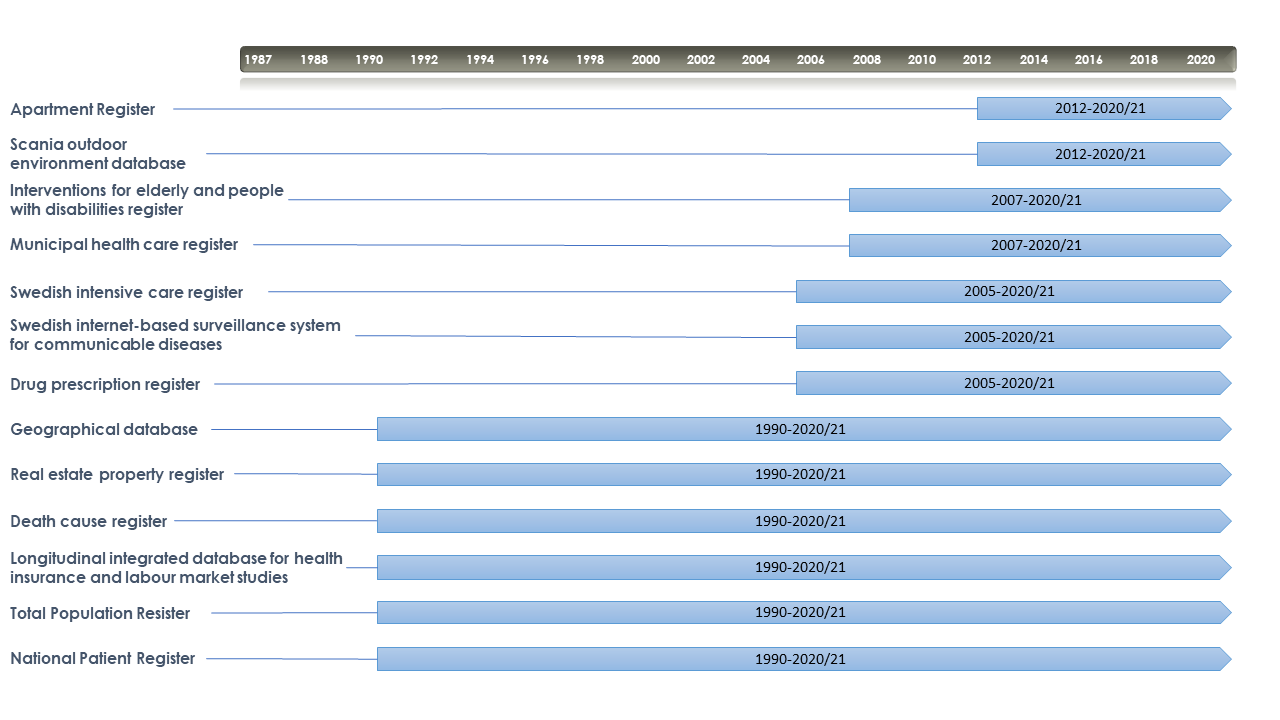
\includegraphics[width=1\linewidth]{output/figures/registers_timeline}

\label{tab:unnamed-chunk-3}Register descriptions

Register

Description

Total Population Register (TPR) (1968)

Sex; birth date; civil status (duration, dates, changes); address (dates, changes); income; country of origin; citizenship; in-/emigration (dates); n of people in the dwelling; housing tenure; socioeconomic indicators of the neighbourhoods (on postal code, municipal levels)

National Patient Register (NPR) (1987)

Hospitalization outcomes: total no. of hospitalizations/month; in-patient health outcomes based on ICD-10 chapters (e.g., for falls, fractures, stroke etc.)

Real Estate Property Register (REPR) (1908)

Objective housing characteristics for each dwelling: type of dwelling; price of dwelling; type of tenure; size; presence of stairs/elevator; floor; building and construction year; characteristics of the neighbourhood: communal facilities (e.g., roads), green areas; date of each relocation

Geographical database (GD) (1952)

DESO (demographical statistical unit); coordinates of the housing and address etc.

Death Cause Register (DR) (1952)

Death cause and date

Longitudinal integrated database for health
insurance and labour market studies (LISA) (1990)

Education level, income, social insurance

Drug Prescription Register (DPR) (2005)

Drug prescriptions for chronic illnesses (ATC code, dose and date): endocrine; cardiovascular; hepatic; renal or neurological/ neuromuscular

Swedish Intensive Care Register (SIRI) (2001)

Intensive care for laboratory-confirmed influenza and (since 2020) COVID-19.

Swedish internet-based surveillance system for communicable diseases (SmiNet) (1997; 2004)

Laboratory-confirmed influenza and (since 2020) COVID-19

Municipal Health Care Register (MHCR) (2007)

Care received and date

Interventions for Elderly and People with Disabilities Register (IEPDR) (2007)

Home help and service type and no of hours/month/year: escorting, replace the relative, personal care, meal delivery, security alarm, daytime activities; short-term vs long-term

Apartment Register (AR) (2012)

Dwelling type; number of rooms; dwelling unit size; kitchen type

Scania Outdoor Environment Database (ScOut)

24 outdoor environemtn qualities 2008-2019

\hypertarget{description-of-data-sets-from-scb}{%
\chapter{Description of data sets from SCB}\label{description-of-data-sets-from-scb}}

A significant amount of data from the registrars originates from Statistics Sweden (SCB). This data is delivered in text format (file extension .txt), and is partitioned, for the most part, into individual files separated by both year and grouped data set. While the data contained in this data originates from the specified data Registrars previously outlined, the data is received from SCB consolidated and grouped into various data sets which require further cleaning and processing. These grouped data sets are described below.

\hypertarget{population}{%
\section{Population}\label{population}}

Description of Population data set

\hypertarget{lisa}{%
\section{Lisa}\label{lisa}}

Description of Lisa data set

\hypertarget{housing}{%
\section{Housing}\label{housing}}

Description of Housing data set

\hypertarget{data-cleaning-and-joining-of-raw-data}{%
\chapter{Data cleaning and joining of raw data}\label{data-cleaning-and-joining-of-raw-data}}

As illustrated above, the data from RELOC-AGE is comprised of from several registers and sources. In order to arrive at the final data set, a number of data cleaning actions, multiple joins, and many quality control steps have been taken to insure reliable analysis and data integrity. This section details steps taken.

\hypertarget{scb-data}{%
\section{SCB data}\label{scb-data}}

With data covering about 3 million individuals over decades and with a multitude of variables spread out across hundreds of very large files, the computational effort to complete these tasks are very time intensive, often taking hours for a large merge, with progress occasionally hindered by computational restrictions and small errors which arise in the data cleaning process. With this in mind, detailed documentation, contained both here and alongside code used in the data cleaning, is prioritized to reduce any need to repeat these time-intensive processes.

As a first step, the following initial data cleaning is performed:

\begin{itemize}
\tightlist
\item
  Raw data files are organized into folder structure where each folder contains all data from a particular data set.
\item
  An individual script for each data set is written in R that reads the raw yearly .txt files and merges files into one data set.
\item
  When required, a variable ``year'' is generated in the joined data set specifying which year the data originates from( taken from the name of the .txt file).
\item
  Variables are renamed into lowercase with spaces and other delimiters transformed into underscores ( \_ ) for consistent naming conventions and avoidance of future merge conflicts.
\item
  The joined and cleaned data set is saved in the contained folder in both R's .rds and Stata's .dta formats.
\item
  A README.txt file is created in each folder documenting the process.
\end{itemize}

The result consists of eleven folders each containing a data set's respective raw data, a documented R merging/cleaning script for full reproducibility, and a merged data set in both R and Stata format to be used in subsequent merging and further analysis.

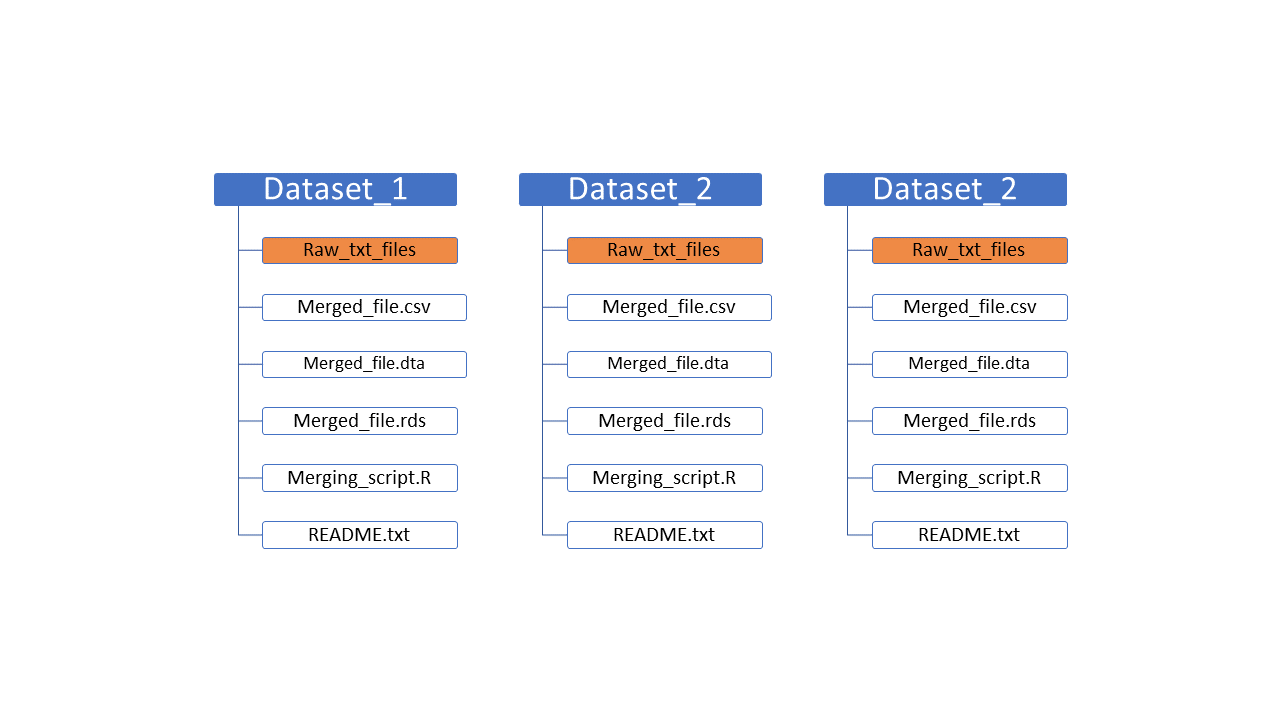
\includegraphics[width=1\linewidth]{output/figures/folder_structure}

\hypertarget{descriptives-by-age-and-sex}{%
\chapter{Descriptives by Age and Sex}\label{descriptives-by-age-and-sex}}

\hypertarget{housing-data}{%
\chapter{Housing data}\label{housing-data}}

Study period 2012-2020 when data is made available from SCB from the Real estate and Apartment registers. Data is taken from three SCB data sources: lev\_lisa, lev\_housing, and lev\_population. The following steps are taken to arrive at a complete data set:

\begin{itemize}
\item
  The unique identifier \textbf{lopnr} in the lev\_population data set is filtered with the following criteria: index\_p ==1 \& ater\_pnr == 0 \& sen\_pnr == 1.
\item
  Next this set of unique identifiers are matched to the full lev\_lisa data set, resulting in lisa data that contains only the unique identifiers from the first step.
\item
  690 duplicate lopnr-year observations are identified and removed from the data set. Further inspection indicated this small number is a result of messy data, showing no trend or further information.
\item
  As data from lev\_lisa ends in 2019 and data from the lev\_housing data set ends in 2020, time invariant variables(year of birth, sex, education, etc.) from unique individuals in 2019 are replicated for 2020 to facilitate the appropriate matching to the unique identifiers in the 2020 Housing data.
\item
  Lastly, the data is joined by the unique lopnr-year combination with the lev\_housing data.
\end{itemize}

\hypertarget{specific-data-considerations}{%
\section{Specific data considerations}\label{specific-data-considerations}}

\hypertarget{identifying-partners}{%
\subsection{Identifying partners}\label{identifying-partners}}

There are some discrepancies in the data when finding consistent partner matches to unique individuals across the multiple data sets.

We can find partner data in two of the datasets: \textbf{partners\_rtb} and \textbf{samh}. In the \textbf{partners\_rtb} dataset, we have three variables for every lopnr-year observation:

\begin{itemize}
\tightlist
\item
  Lopnrsamh -- (no definition given in the excel sheet) 1987-1997.
\item
  Lopnrsambo -- ``sambo's personummer'' from 1998.
\item
  Lopnrmakpart -- ``make/maka/partners personummer'' ( I believe this is technically married) from 1998.
\end{itemize}

From the \textbf{samh} dataset, we have one variable:
* LopNrSamh -- (no definition given in the accompanying excel sheet).

Since no particular partner variable was consistent over time, a new varaible is created, ``partner'', that takes the value of whichever variable has valid data (of one of the above variables) for that lopnr/year. If there are two values, the priority is for the lopnrsamh from the \textbf{partners\_rtb} dataset (it seems to have the best coverage).

A screenshot for an particular individual with multiple partners over time to illustrate.

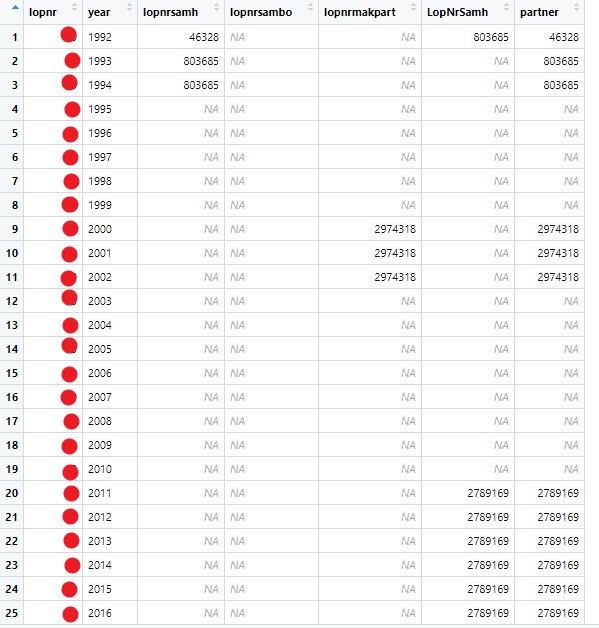
\includegraphics[width=0.8\linewidth]{output/figures/partners_png}

\hypertarget{recoding-varaibles}{%
\subsection{Recoding varaibles}\label{recoding-varaibles}}

Education, housing type, housing tenure

\hypertarget{indentifying-relocations}{%
\subsection{Indentifying relocations}\label{indentifying-relocations}}

To identify when an individual has relocated in the data the following considerations are taken into account.

\begin{itemize}
\tightlist
\item
  The housing variables, \textbf{fast\_lopnr} and \textbf{lghlopnr} appear to uniquely identify the housing location of a particular individual. Over time, a change in either variable should indicate that an individual as relocated (highlighted in orange below). This change appears to be the best indicator of whether an individual has relocated or not.
\end{itemize}

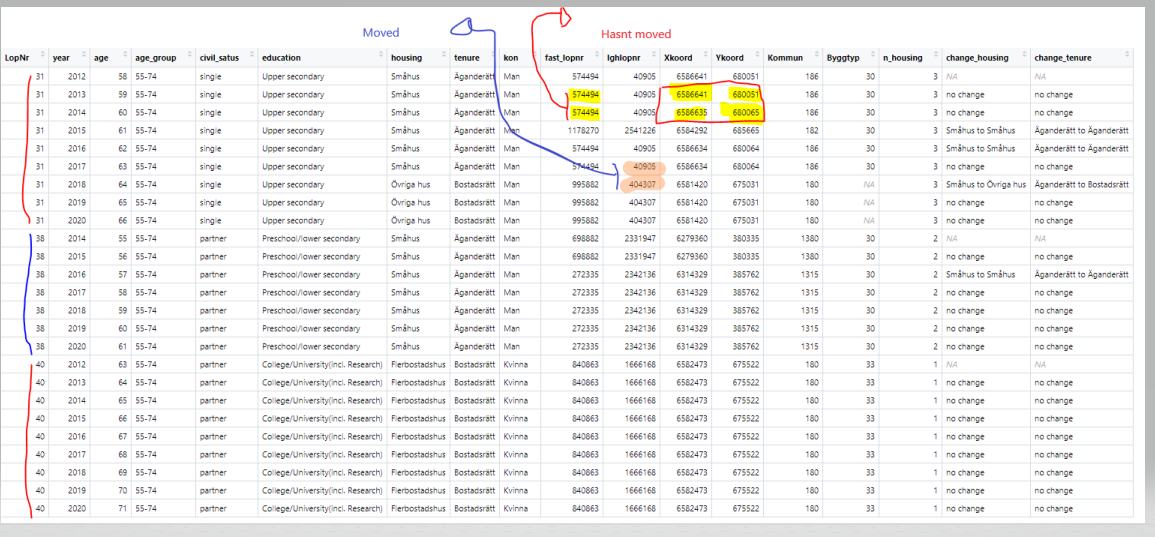
\includegraphics[width=1\linewidth]{output/figures/relocation_id}

\begin{itemize}
\item
  The coordinate variables, \textbf{xkoord} and \textbf{ykoord} appear to be occasionally inconsistent, giving different values for the same \textbf{fast\_lopnr} and \textbf{lghlopnr} identifier in some of the data. This may be the result of data errors or possibly a GPS margin of error when measuring housing location (Highlighted yellow).
\item
  The variable \textbf{n\_housing} counts how many unique \textbf{fast\_lopnr}'s are associated with each \textbf{lopnr}. For example, individual RED, has resided in three locations, Individual BLUE has resided in two locations, and Individual 40 has resided in one location during the sample period.
\item
  The vairalbes \textbf{change\_housing} and \textbf{change\_tenure} take the before and after values of \textbf{housing} and \textbf{tenure} (respectively) and return the before and after categories when a change (relocation) has occurred.
\item
  \textbf{Byggtyp} appears to follow the patterns of \textbf{fast\_lopnr} and \textbf{lghlopnr}, but contains some missing data. The missing \textbf{Byggtyp} value seems to be associated with the values ``Övriga hus'' and ``Specialböstader'' in \textbf{housing}.
\end{itemize}

\hypertarget{indentifying-change-in-kommun}{%
\subsection{Indentifying change in kommun}\label{indentifying-change-in-kommun}}

In a similar fashion as identifying the change in a housing identifier over time for an individual, we can observe when an individual has relocated outside of a geographical area when the geographical indicator changes.

\end{document}
